\documentclass[aspectratio=169, 10pt]{beamer}
\usepackage[utf8]{inputenc}
\usepackage{graphicx}
\usepackage[portuguese]{babel}
\usepackage{utopia} %font utopia imported
\usepackage{ragged2e}
\usetheme{Boadilla}
\usecolortheme{dolphin}
\usepackage[alf]{abntex2cite}

%\usepackage[colorlinks = true,
%            linkcolor = black,
%            urlcolor  = black,
%            citecolor = blue,
%            anchorcolor = yellow]{hyperref}

% set colors
\definecolor{myNewColorA}{RGB}{45, 75, 115}
\definecolor{myNewColorB}{RGB}{37, 60, 89}
\definecolor{myNewColorC}{RGB}{153, 180, 191}
\definecolor{deepmagenta}{rgb}{0.8, 0.0, 0.8}

%% I use a beige off white for my background
%\definecolor{MyBackground}{RGB}{255,253,218}

\setbeamercolor*{palette primary}{bg=myNewColorC}
\setbeamercolor*{palette secondary}{bg=myNewColorB, fg = white}
\setbeamercolor*{palette tertiary}{bg=myNewColorA, fg = white}
\setbeamercolor*{titlelike}{fg=myNewColorA}
\setbeamercolor{footline}{fg = white}%, bg = black}

%% Uncomment this if you want to change the background color to something else
%\setbeamercolor{background canvas}{bg=MyBackground}

\setbeamercolor*{item}{fg=myNewColorA}
\setbeamercolor*{caption name}{fg=myNewColorA}
\usefonttheme{professionalfonts}
%\usepackage{natbib}
\usepackage{hyperref}
\hypersetup{
    colorlinks = true,
    linkcolor = blue,
    citecolor= blue
}
%------------------------------------------------------------
\titlegraphic{
\includegraphics[height=1.5cm]{UFPE.png}} 

\setbeamerfont{title}{size=\Large}
\setbeamerfont{subtitle}{size=\small}
\setbeamerfont{author}{size=\small}
\setbeamerfont{date}{size=\small}
\setbeamerfont{institute}{size=\small}
\title[\textcolor{white}{Incerteza - Estados Brasileiros}]{Impactos da Incerteza sobre a atividade econômica dos estados brasileiros}
%\subtitle{ }
\author[Silva Junior]{Paulo Francisco da Silva Júnior}

\institute[UFPE]{Universidade Federal de Pernambuco}
\date[\textcolor{white}{10 de abril de 2025}]
{10 de Abril de 2025}




%------------------------------------------------------------
%This block of commands puts the table of contents at the 
%beginning of each section and highlights the current section:
%\AtBeginSection[]
%{
%  \begin{frame}
%    \frametitle{Contents}
%    \tableofcontents[currentsection]
%  \end{frame}
%}

\AtBeginSection[]{
  \begin{frame}
  \vfill
  \centering
  \begin{beamercolorbox}[sep=8pt,center,shadow=true,rounded=true]{title}
    \usebeamerfont{title}\insertsectionhead\par%
  \end{beamercolorbox}
  \vfill
  \end{frame}
}
%------------------------------------------------------------

\begin{document}

%The next statement creates the title page.
\frame{\titlepage}
\begin{frame}
\frametitle{Conteúdo}
\tableofcontents
\end{frame}
%------------------------------------------------------------
\justifying

\section{Introdução}
\begin{frame}{Introdução}
\begin{itemize}
    \item Desde a recessão financeira de 2008-2009, há um crescimento da literatura para compreensão do choque de incerteza sobre o ciclo dos negócios.
    \item Um choque de incerteza produz, em geral, efeitos negativos \cite{haddow2013macroeconomic, bloom2014fluctuations}, porém os impactos variam entre os países \cite{bloom2017observations}. 
    \item Em complemento, \citeonline{mumtaz2018does, mumtaz2018stateimpact, silva2024effects} mostram que as respostas são heterogêneas entre os estados dos EUA.
    \item Para o caso brasileiro, como nos estudos de \citeonline{costa2014incerteza} e \citeonline{barboza2018efeitos}, existem evidências apenas para o nível agregado.
    \item Dessa forma, esse trabalho tem o objetivo de:
    \begin{itemize}
        \item identificar se há reações heterogêneas entre os estados Brasileiros
        \item compreender as respostas dos estados a partir de características econômicas estruturais
    \end{itemize}
\end{itemize}
\end{frame}

\section{Revisão de literatura}
\begin{frame}{Revisão de literatura}
%\begin{columns}[c]
%\begin{column}{.5\textwidth}
Sobre incerteza
\begin{itemize}
    \item Definição moderna por \citeonline{knight1921risk}: risco trata-se de uma probabilidade conhecida, mas para a incerteza, a probabilidade é desconhecida;
    \item Dificuldade de mensuração: uso de \textit{proxies}, por exemplo, variações de indicadores econômicos e previsões de mercado, citações de jornais referente a incerteza, etc \cite{FMI2012outlook, bloom2014fluctuations}.
     \item Impacto negativo sobre consumo, investimento, produção, crédito e produtividade \cite{haddow2013macroeconomic}. 
     %Pode ser positivo se houver benefício líquido de investir \cite{bernanke1983irreversibility, bloom2014fluctuations}
\end{itemize}
Por quê incerteza importa?
\begin{itemize}
    \item World Economic Outlook (2012): impacto doloroso na atividade econômica; um dos principais fatores que retardou a recuperação da crise global financeira em 2008-2009 \cite{FMI2012outlook}.
    \item Causalidade e identificação é um desafio \cite{baker2016measuring, ludvigson2021uncertainty}.
     \item Necessário entendimento da dinâmica do choque de incerteza para o desenvolvimento de políticas que mitiguem os impactos negativos \cite{haddow2013macroeconomic}.  
\end{itemize}

\end{frame}

\begin{frame}{Revisão de literatura}
Diferenças regionais
\begin{itemize}
    \item Incerteza varia entre regiões:
    \begin{itemize}
        \item países em desenvolvimento sofrem mais impacto externo \cite{bloom2017observations}.
        \item os estados dos EUA apresentam respostas heterogêneas que estão relacionadas à características estruturais como: concentração de setores, relação de gastos e abertura comercial \cite{mumtaz2018does, mumtaz2018stateimpact, silva2024effects}.
   \end{itemize}
\end{itemize}
Evidência para o Brasil
\begin{itemize}
    \item Principais trabalhos: \citeonline{costa2014incerteza} e \citeonline{barboza2018efeitos}.
     \item Produção industrial mais afetada que o PIB;
     \item \citeonline{barboza2018efeitos} sugere que há componentes do PIB que não sejam tão afetados pela incerteza doméstica quanto a indústria.
     \item Incerteza doméstica é mais significativa que incerteza externa;
\end{itemize}
\end{frame}

\section{Metodologia}
\subsection{Dados}
\begin{frame}{Dados}
Para o modelo SVAR:
\begin{itemize}
    \item Período de Jan/2004 até Dez/2019, com frequência mensal, e total de 192 observações.
    \item Estados: Bahia (BA), Ceará (CE), Espírito Santo (ES), Goiás (GO), Minas Gerais (MG), Pará (PA), Paraná (PR), Pernambuco (PE), Rio de Janeiro (RJ), Rio Grande do Sul (RS), Santa Catarina (SC) e São Paulo (SP). 
    \item Medidas de incerteza:
        \begin{itemize}
            \item Indicador de Incerteza Econômica - Brasil (IIE-Br)
            \item Economic Policy Uncertainty (EPU) para o Brasil
            \item Global Economic Policy Uncertainty (GEPU)
        \end{itemize}
    \item Índice de Atividade Econômica Regional (IBCR) desazonalizado.
    \item Pesquisa Industrial Mensal - Produção Física (PIM) desazonalizado.
    \item Índice de emprego formal (IEF). Ajuste sazonal realizado com X-13 ARIMA.
    \item Média mensal do fechamento diário do Ibovespa.
    \item Média mensal da taxa Selic Meta.
 \end{itemize}
\end{frame}

\begin{frame}{Dados}
Para o modelo cross-section:
\begin{itemize}
    \item Densidade demográfica da tabela 4714 do senso demográfico
de 2022 - IBGE;
    \item Demais dados estão entre o período de 2016 até 2019, com frequência anual:
        \begin{itemize}
            \item Exportações e importações estaduais. Portal ComExStat. 
            \item PIB Estadual - preços de mercado (preços de 2010);
            \item PIB Estadual (valor adicionado a preços básico) agropecuária (preços de 2010);
            \item PIB Estadual (valor adicionado a preços básicos) -
indústria - construção civil (preços de 2010);
            \item PIB Estadual (valor adicionado a preços básicos) - indústria - extrativa (preços de 2010); 
            \item PIB Estadual (valor adicionado a preços
básicos) - indústria - transformação (preços de 2010); 
            \item PIB Estadual (valor adicionado a preços básicos) - serviços - administração, defesa, saúde e educação públicas e seguridade social (preços de 2010); 
            \item PIB Estadual (valor adicionado a preços básicos) - serviços - atividades financeiras, de seguros e serviços relacionados (preços de 2010); 
            \item Despesa corrente - empenhada - estadual;
        \end{itemize} 
 \end{itemize}
\end{frame}

\subsection{Modelos}
\begin{frame}{Modelo - SVAR}
Formalmente o modelo SVAR base utilizado é especificado pelo seguinte
formato:
\begin{equation}
\label{eq:model_1}
    B_{b}Y_{t,b}=C_{b}+\sum_{i=1}^{N} {C_{i,b}Y_{t-i,b}} + U_{t,b}
\end{equation}
onde para cada estado $b$ é estimado:
\begin{enumerate}
    \item[] $Y_{t,b}$, um vetor coluna 5x1 das variáveis endógenas do modelo;
    \item[] $B_{b}$, uma matriz 5x5 dos efeitos contemporâneos;
    \item[] $C_b$, um vetor coluna 5x1 de termos constantes;
    \item[] $C_{i,b}$, uma matriz 5x5 dos efeitos defasados;
    \item[] $U_{t,b}$, um vetor coluna 5x1 dos choques estruturais;
\end{enumerate}
até $N$ defasagens, utilizando decomposição Cholesky com 1's na diagonal principal. 
\newline\newline
Ordenação causal: Incerteza, log(Ibovespa), Selic, log(Emprego), log(Atividade Econômica).
\end{frame}

\begin{frame}{Modelo - Cross section}
Formalmente o modelo cross section está definido como:

\begin{equation}
\label{eq:model_2}
    IRF^{t}_{i} = \beta_{0} + \beta_{1}X_{i} + u
\end{equation}
onde para cada estado i, é calculado:
\begin{itemize}
    \item $IRF^{t}_{i}$, o impacto absoluto no período t do estado i; \textsuperscript{1}
    \item $\beta_{0}$, um termo constante;
    \item $\beta_{1}$, um vetor de coeficientes em resposta ao vetor $X_{i}$;
    \item $X_{i}$,  um vetor de \textit{proxies} para capturar as características estruturais do estado i;
    \item $u$ o termo de erro da equação;
\end{itemize}
\vfill
\tiny \textsuperscript{1} Foi escolhida a resposta absoluta do 9\textordmasculine\ período da medida de incerteza IIE-Br, pois apresenta o maior impacto de incerteza, juntamente com a medida IBCR, com o objetivo de capturar todos os setores relacionados a produção.
\end{frame}

\section{Resultados}
\subsection{SVAR}
\begin{frame}{Resultados - IIE-Br}
\vspace{-1.5em}
\begin{figure}[htb!]
    \caption{\footnotesize Respostas do IBCR após um choque da medida de incerteza IIE-Br}\vspace{-0.75em}
    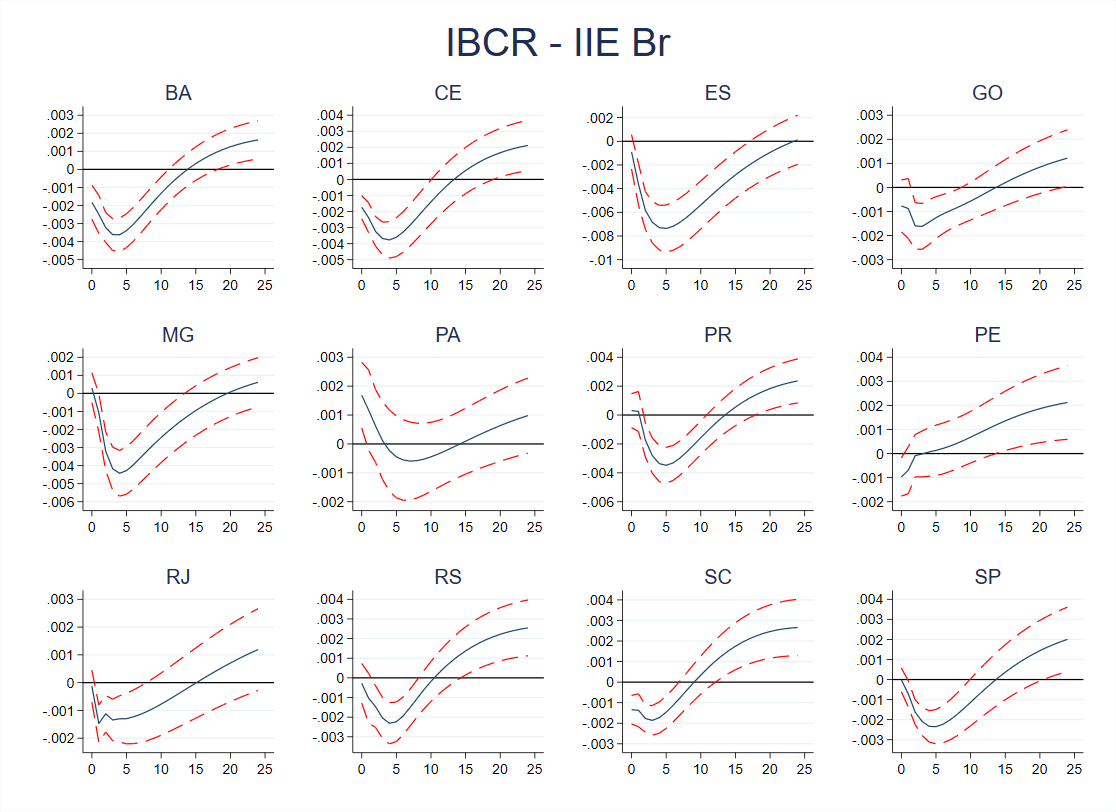
\includegraphics[height=0.8\textheight]{Figs/IRF/IRF_IIE_IBCR.png}
\end{figure}
\vspace{-1.25em}
\tiny Fonte: Elaboração própria. Nota: Respostas estaduais após o choque de um desvio padrão na medida de incerteza. Os números do gráfico estão descritos em valores absolutos. A linha tracejada em vermelho representa o intervalo de confiança de 68\%.
\end{frame}

\begin{frame}{Resultados - IIE-Br}
%\begin{columns}
%\begin{column}{.5\textwidth}
\vspace{-1.5em}
%\begin{figure}[htb!]
    %\caption{\footnotesize Respostas do IBCR após um choque da medida de incerteza IIE-Br}
    %\vspace{-1.75em}
    %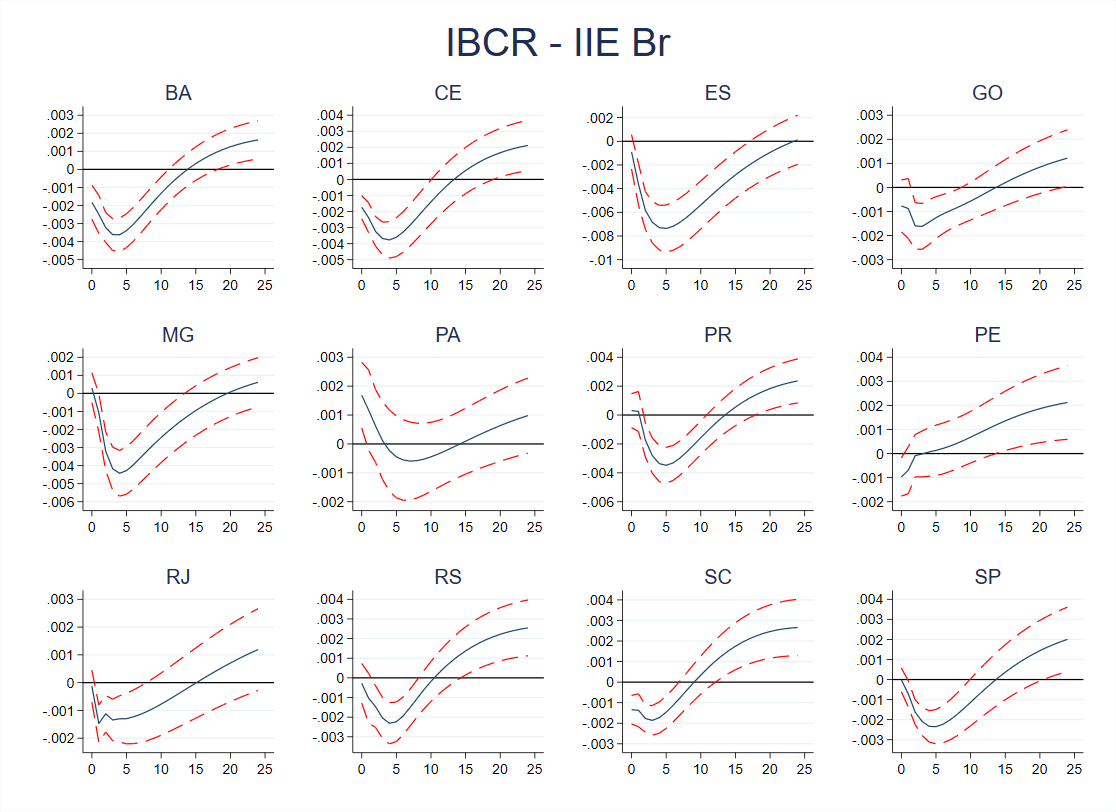
\includegraphics[height=0.65\textheight]{Figs/IRF/IRF_IIE_IBCR.png}
    %\label{fig:IRF_IIE_IBCR}
    %\footnotesize
%Fonte: Elaboração própria. Nota: Respostas estaduais após o choque de um desvio padrão na medida de incerteza. Os números do gráfico estão descritos em valores absolutos. A linha tracejada em vermelho representa o intervalo de confiança de 68\%.
%\end{figure}
%\end{column}
%\begin{column}{.5\textwidth}
%\vspace{-1em}
\begin{figure}[htb!]
    \caption{\footnotesize Respostas da PIM após um choque da medida de incerteza IIE-Br}
    \vspace{-0.75em}
    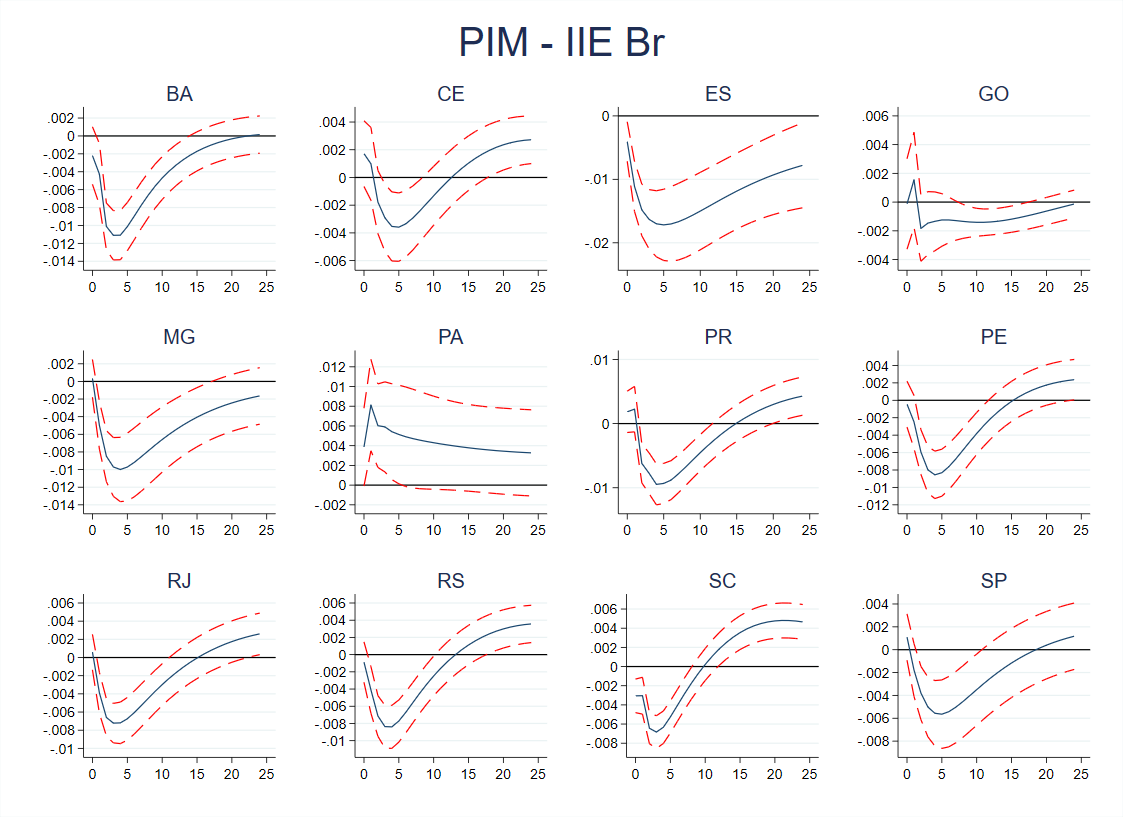
\includegraphics[height=0.8\textheight]{Figs/IRF/IRF_IIE_PIM.png}
    \label{fig:IRF_IIE_PIM}
\end{figure}
%\end{column}
%\end{columns}
\vspace{-1.25em}
\tiny Fonte: Elaboração própria. Nota: Respostas estaduais após o choque de um desvio padrão na medida de incerteza. Os números do gráfico estão descritos em valores absolutos. A linha tracejada em vermelho representa o intervalo de confiança de 68\%.
\end{frame}

\begin{frame}{Resultados - EPU-Br}
\vspace{-1.5em}
\begin{figure}[htb!]
    \caption{\footnotesize Respostas do IBCR após um choque da medida de incerteza EPU-Br}\vspace{-0.75em}
    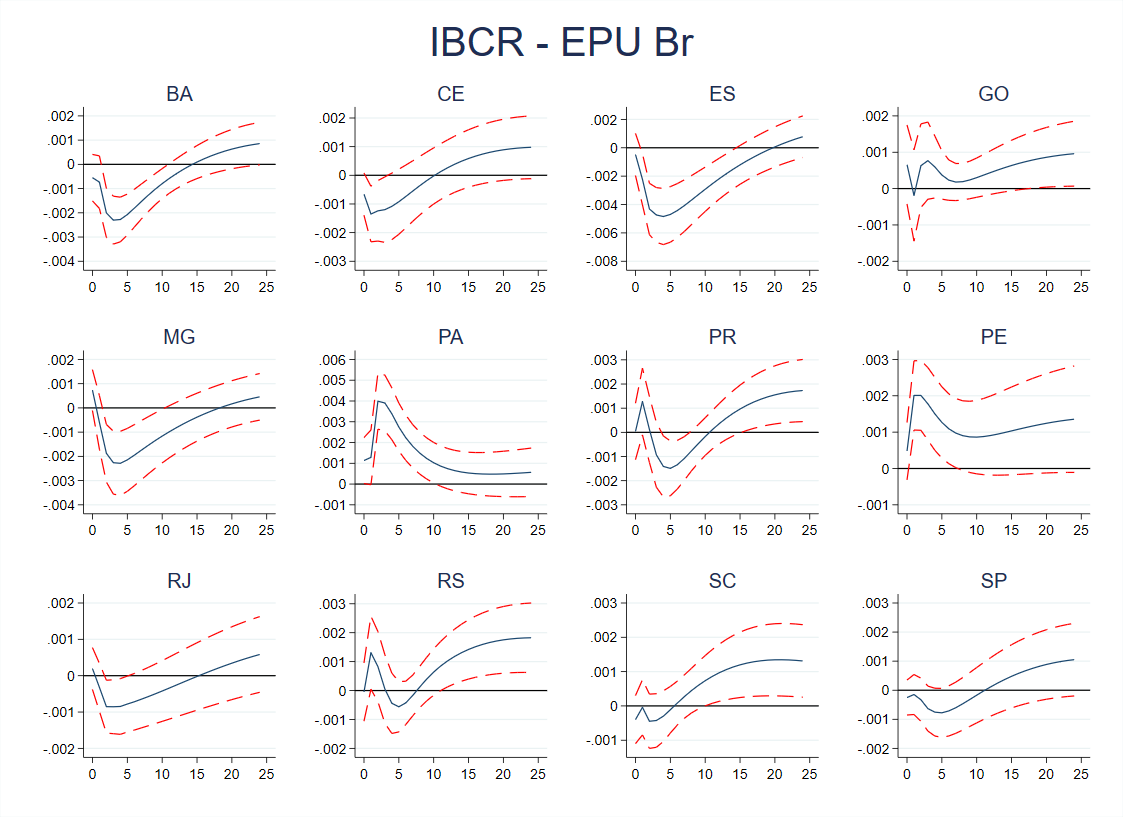
\includegraphics[height=0.8\textheight]{Figs/IRF/IRF_EPU_IBCR.png}
\end{figure}
\vspace{-1.25em}
\tiny Fonte: Elaboração própria. Nota: Respostas estaduais após o choque de um desvio padrão na medida de incerteza. Os números do gráfico estão descritos em valores absolutos. A linha tracejada em vermelho representa o intervalo de confiança de 68\%.
\end{frame}

\begin{frame}{Resultados - EPU-Br}
\vspace{-1.5em}
\begin{figure}[htb!]
    \caption{\footnotesize Respostas da PIM após um choque da medida de incerteza EPU-Br}\vspace{-0.75em}
    \begin{center}
        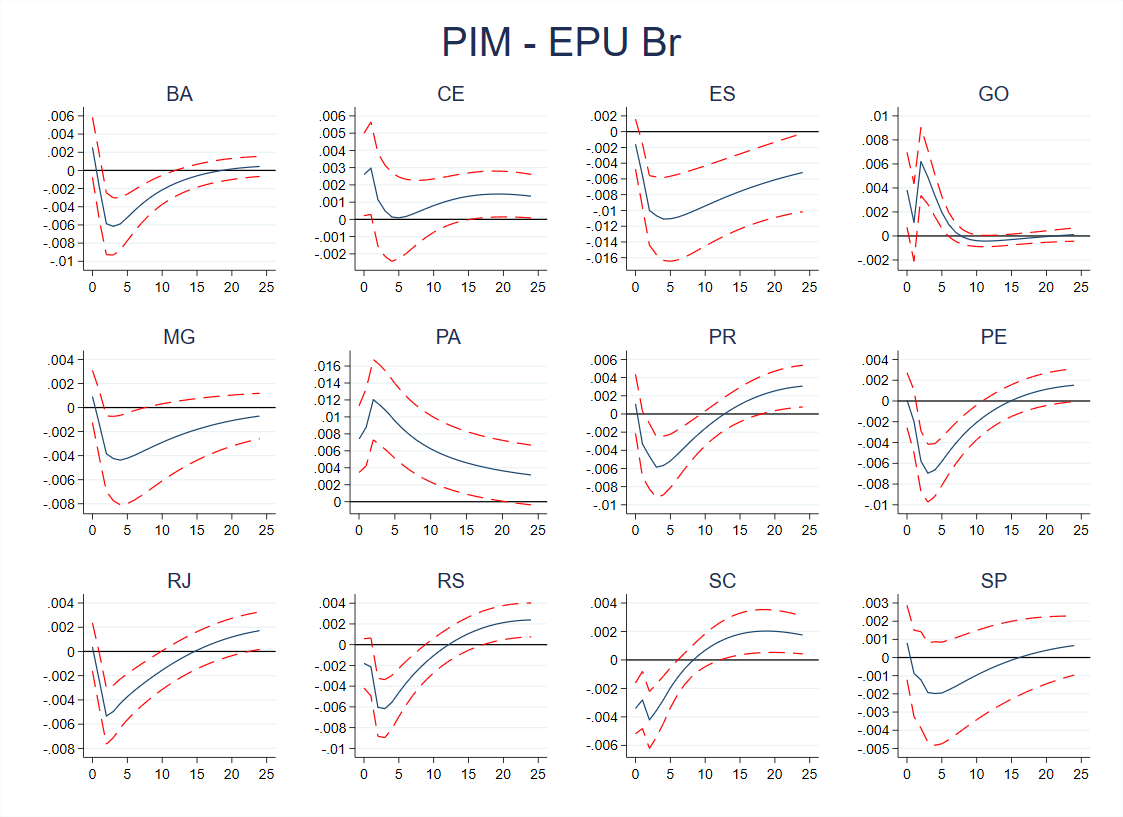
\includegraphics[height=0.8\textheight]{Figs/IRF/IRF_EPU_PIM.png}
    \end{center}
\end{figure}
\vspace{-1.25em}
\tiny Fonte: Elaboração própria. Nota: Respostas estaduais após o choque de um desvio padrão na medida de incerteza. Os números do gráfico estão descritos em valores absolutos. A linha tracejada em vermelho representa o intervalo de confiança de 68\%.
\end{frame}

\begin{frame}{Resultados - GEPU}
\vspace{-1.5em}
\begin{figure}[htb!]
    \caption{\footnotesize Respostas do IBCR após um choque da medida de incerteza GEPU}\vspace{-0.75em}
    \begin{center}
        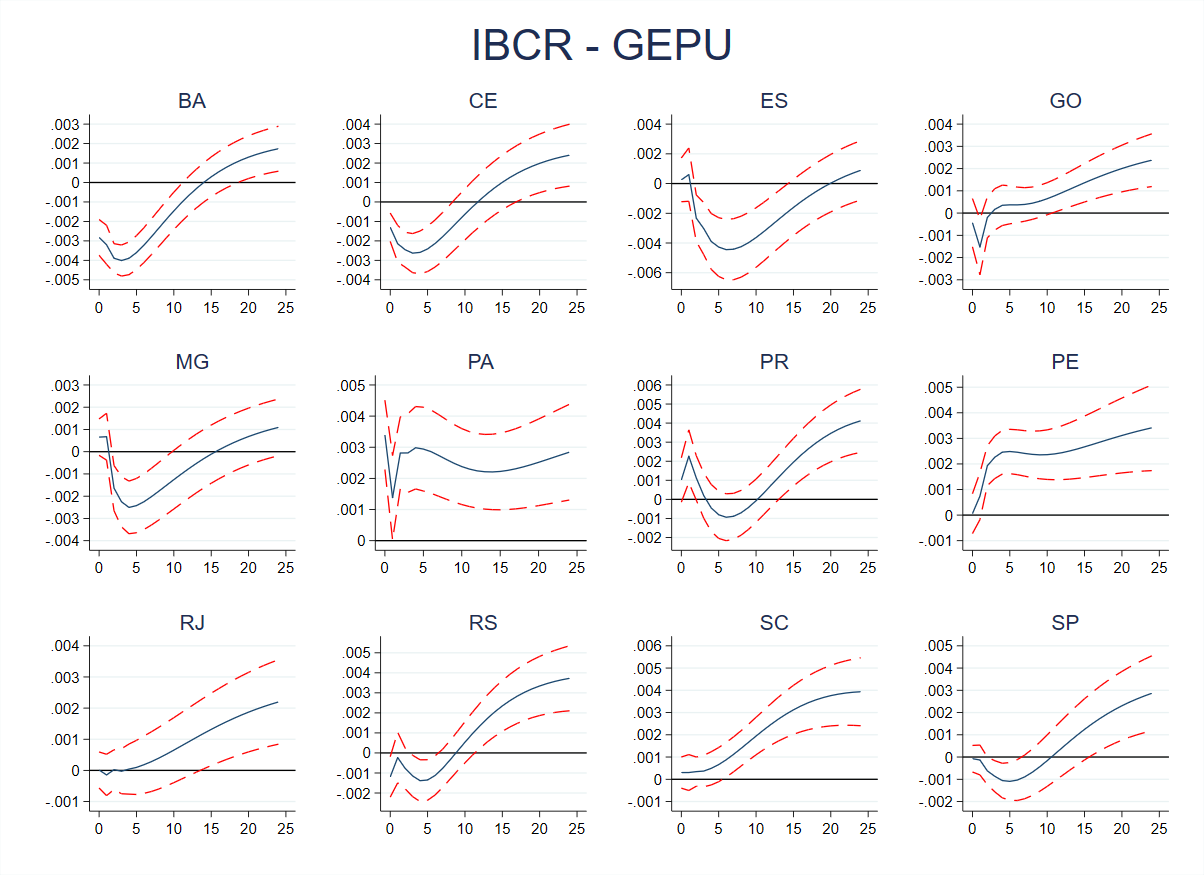
\includegraphics[height=0.8\textheight]{Figs/IRF/IRF_GEPU_IBCR.png}
    \end{center}
\end{figure}
\vspace{-1.25em}
\tiny Fonte: Elaboração própria. Nota: Respostas estaduais após o choque de um desvio padrão na medida de incerteza. Os números do gráfico estão descritos em valores absolutos. A linha tracejada em vermelho representa o intervalo de confiança de 68\%.
\end{frame}

\begin{frame}{Resultados - GEPU}
\vspace{-1.5em}
\begin{figure}[htb!]
    \caption{\footnotesize Respostas da PIM após um choque da medida de incerteza GEPU}\vspace{-0.75em}
    \begin{center}
        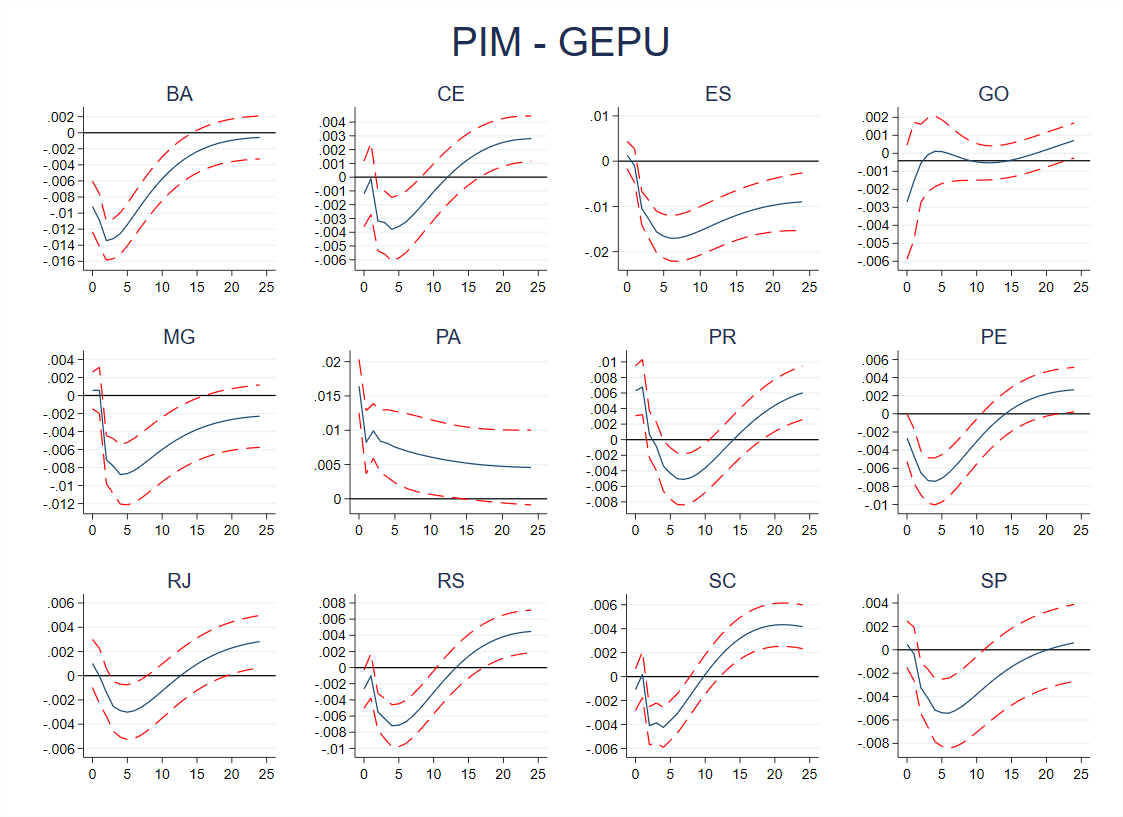
\includegraphics[height=0.8\textheight]{Figs/IRF/IRF_GEPU_PIM.png}
    \end{center}
\end{figure}
\vspace{-1.25em}
\tiny Fonte: Elaboração própria. Nota: Respostas estaduais após o choque de um desvio padrão na medida de incerteza. Os números do gráfico estão descritos em valores absolutos. A linha tracejada em vermelho representa o intervalo de confiança de 68\%.
\end{frame}

\subsection{Robustez}
\begin{frame}{Resultados - Robustez} \label{section:robustez_slide}
Para o exercício de robustez\textsuperscript{1} do modelo foram implementadas as variações abaixo:

\begin{enumerate}
    \item[1] Inclusão de tendência
    \item[2] Exclusão da série de emprego
    \item[3] Exclusão da série Ibovespa
    \item[4] Ordenação causal: Atividade, Emprego, Selic, Incerteza, Ibovespa
    \item[5] Ordenação causal: Incerteza, Atividade, Emprego, Selic, Ibovespa
    \item[6] Ordenação causal: Atividade, Emprego, Selic, Ibovespa, Incerteza
\end{enumerate}
Em geral, robustos, porém ressalva em alguns casos. \newline
Ressalva baseada nas diferenças de: intensidade do choque, dinâmica de reação e taxa de recuperação da atividade econômica. \newline
\vfill \tiny \textsuperscript{1} Os gráficos do exercício de robustez podem ser consultados no apêndice - \ref{section: Robustness}.
\end{frame}

\subsection{Cross section}
\begin{frame}{Resultados - Cross section}
\tiny
\vspace{-1.75em}
\begin{center}
\begin{table}[htb!]
\caption{Resultados da regressão cross section}
\label{table:cross_section_results}
\vspace{-0.5em}
\tiny
\begin{tabular}{l c c c c c c
    %>{\centering\arraybackslash}m{0.5cm}
    %>{\centering\arraybackslash}m{1.5cm}
    %>{\centering\arraybackslash}m{1.25cm}
    %>{\centering\arraybackslash}m{1.5cm}
    %>{\centering\arraybackslash}m{1.25cm}
    %>{\centering\arraybackslash}m{2.25cm}
    %>{\centering\arraybackslash}m{2.25cm}
    %>{\centering\arraybackslash}m{2.25cm}
    }
  \hline
& Modelo 1 & Modelo 2 & Modelo 3 \\
  \hline
Agropecuária & 0.0684*** & 0.0395 & 0.0764* \\
 & (0.0175) & (0.0299) & (0.0209) \\
Construção Civil & -0.1447 & -0.1722 & -0.0477 \\
 & (0.0933) & (0.0924) & (0.0670) \\
Indústria Extrativa & 0.0373 & 0.0013 & 0.0362 \\
 & (0.0192) & (0.0360) & (0.0232) \\
Indústria de Transformação & 0.1170** & 0.1332** & 0.1341** \\
 & (0.0332) & (0.0347) & (0.0190) \\
Serviços Financeiros & 0.1615** & 0.1563** & 0.1534** \\
 & (0.0420) & (0.0405) & (0.0222) \\
Serviços Públicos & 0.1612** & 0.1841** & 0.1535** \\
 & (0.0353) & (0.0391) & (0.0240) \\
Grau de endividamento & -0.0488** & -0.0614** & -0.0342 \\
 & (0.0125) & (0.0161) & (0.0130) \\
Grau de Abertura &  & 0.0122 & 0.0030 \\
 &  & (0.0105) & (0.0066) \\ 
Densidade Demográfica &  &  & 0.00001** \\
 &  &  & (0.00000) \\
Constante & -0.0345** & -0.0340** & -0.0437** \\
 & (0.0100) & (0.0096) & (0.0062) \\
\hline
R2 Ajustado & 0.63 & 0.66 & 0.89 \\
Observações & 12 & 12 & 12 \\
\hline
\end{tabular}
\end{table}
\end{center}
\vspace{-0.25em}
\tiny Fonte: Elaboração própria.
Nota: Estão presentes os coeficientes dos modelos com os respectivos erros padrões entre parênteses. Níveis de significância estão descritos como: *** p<0.01; ** p<0.05; e * p<0.10. Esta tabela considera a resposta absoluta do 9\textordmasculine\ período, $IRF_{i}^{9}$, para a estimação.
\end{frame}

\section{Conclusão}
\begin{frame}{Conclusão}
\begin{itemize}
    \item Através do modelo SVAR, nota-se que os estados brasileiros respondem de forma heterogênea a choques de incerteza, com diferentes proporções e trajetórias.
    \item A produção industrial apresenta maior impacto negativo do que a \textit{proxy} do PIB, o IBCR. 
    \item Intensidade do choque: expectativas de mercado > incerteza externa > incerteza interna. 
    \item Os resultados do modelo com corte transversal indicam que os choques estão relacionados a estrutura econômica dos estados. Concentração de setores, grau de endividamento e de abertura.
    \item Estados com maior participação do ramo de construção e alto grau de endividamento, em relação ao PIB, são negativamente afetados.
    \item Já estados com maior concentração de setores como agropecuária, industria extrativa e serviços públicos, tendem a sofrer menos impactos negativos.
\end{itemize}
\end{frame}

\section*{OBRIGADO!}

\section{Referências}
\begin{frame}[allowframebreaks]{Referências}
\footnotesize
%\bibliographystyle{abntex2-alf}
\bibliography{literature}
\end{frame}

\section{Appendix - Robustez} \label{section: Robustness}
\begin{frame}{Robustez - IIE-Br - IBCR}
\begin{figure}[htb!]
    \caption{\footnotesize Robustez - IBCR após um choque da medida de incerteza IIE-Br}
    \begin{center}
        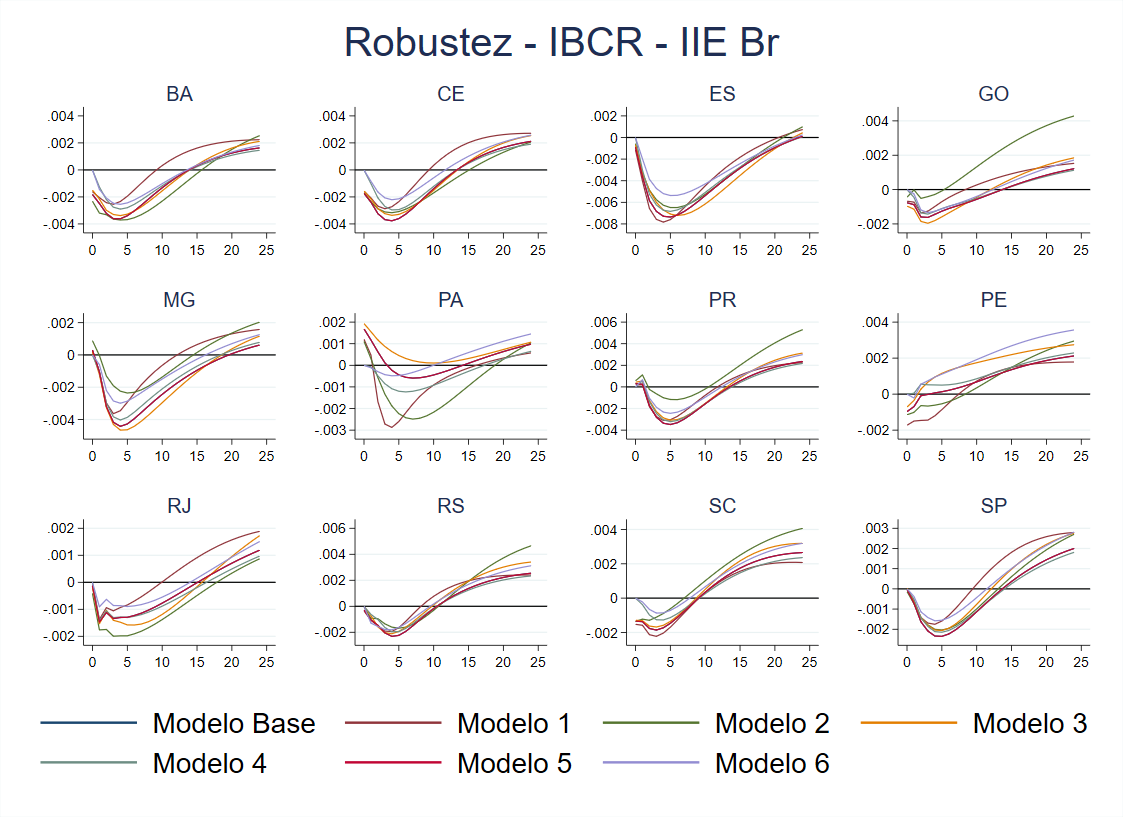
\includegraphics[height=0.65\textheight]{Figs/Robusteness/IRF_IIE_IBCR_robustness.png}
    \end{center}
    \label{fig:IRF_IIE_IBCR_robustness} \footnotesize
Fonte: Elaboração própria. Nota: Respostas estaduais após o choque de um desvio padrão na medida de incerteza. Os números do gráfico estão descritos em valores absolutos. 
\end{figure}
\end{frame}

\begin{frame}{Robustez - IIE-Br - PIM}
\begin{figure}[htb!]
    \caption{\footnotesize Robustez - PIM após um choque da medida de incerteza IIE-Br}
    \begin{center}
        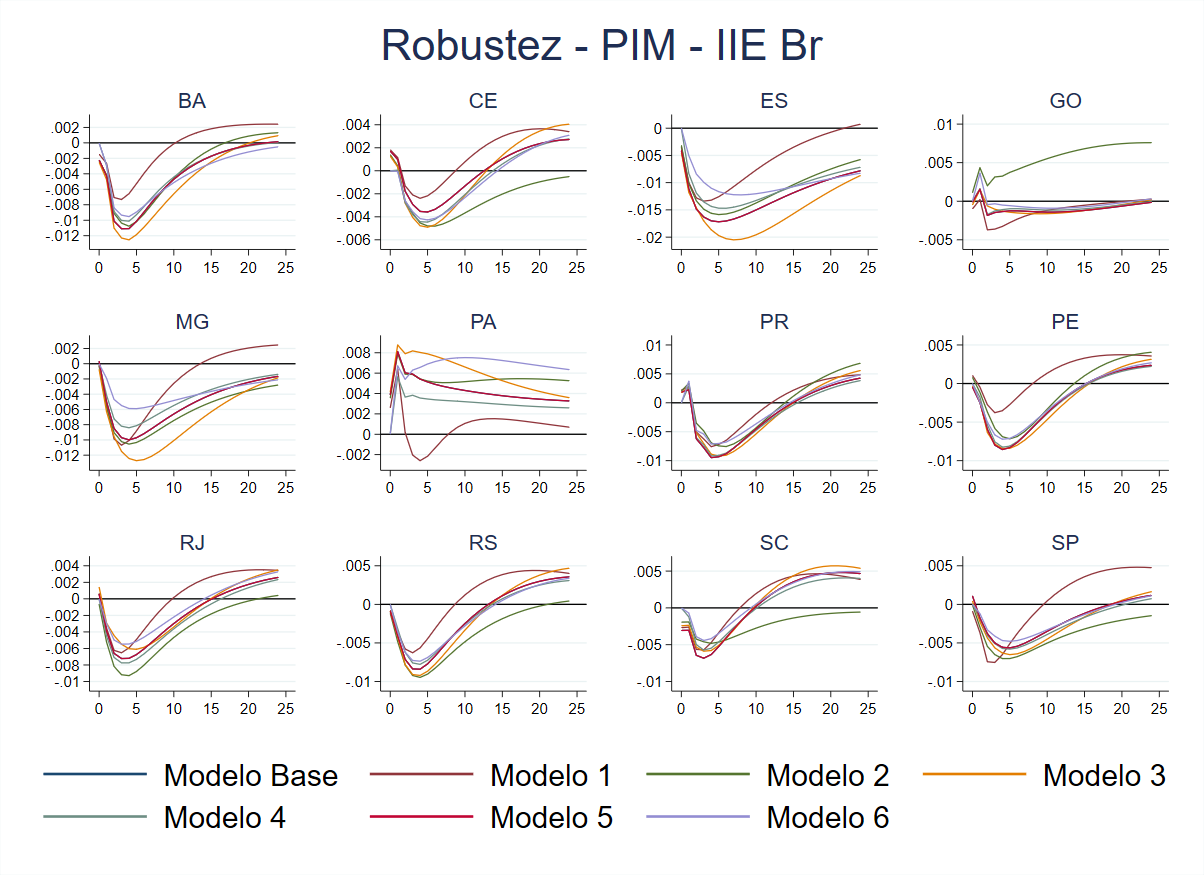
\includegraphics[height=0.65\textheight]{Figs/Robusteness/IRF_IIE_PIM_robustness.png}
    \end{center}
    \label{fig:IRF_IIE_PIM_robustness} \footnotesize
Fonte: Elaboração própria. Nota: Respostas estaduais após o choque de um desvio padrão na medida de incerteza. Os números do gráfico estão descritos em valores absolutos. 
\end{figure}
\end{frame}

\begin{frame}{Robustez - EPU-Br - IBCR}
\begin{figure}[htb!]
    \caption{\footnotesize Robustez - IBCR após um choque da medida de incerteza EPU-Br}
    \begin{center}
        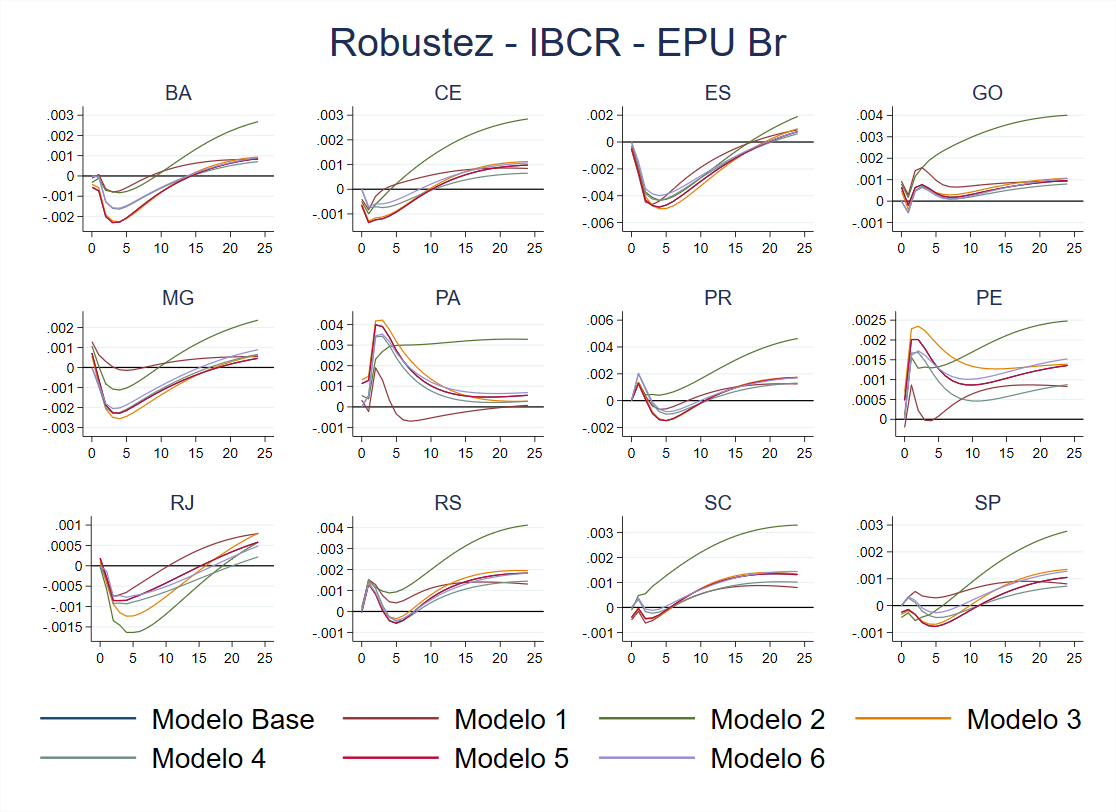
\includegraphics[height=0.65\textheight]{Figs/Robusteness/IRF_EPU_IBCR_robustness.png}
    \end{center}
    \label{fig:IRF_EPU_IBCR_robustness} \footnotesize
Fonte: Elaboração própria. Nota: Respostas estaduais após o choque de um desvio padrão na medida de incerteza. Os números do gráfico estão descritos em valores absolutos. 
\end{figure}
\end{frame}

\begin{frame}{Robustez - EPU-Br - PIM}
\begin{figure}[htb!]
    \caption{\footnotesize Robustez - PIM após um choque da medida de incerteza EPU-Br}
    \begin{center}
        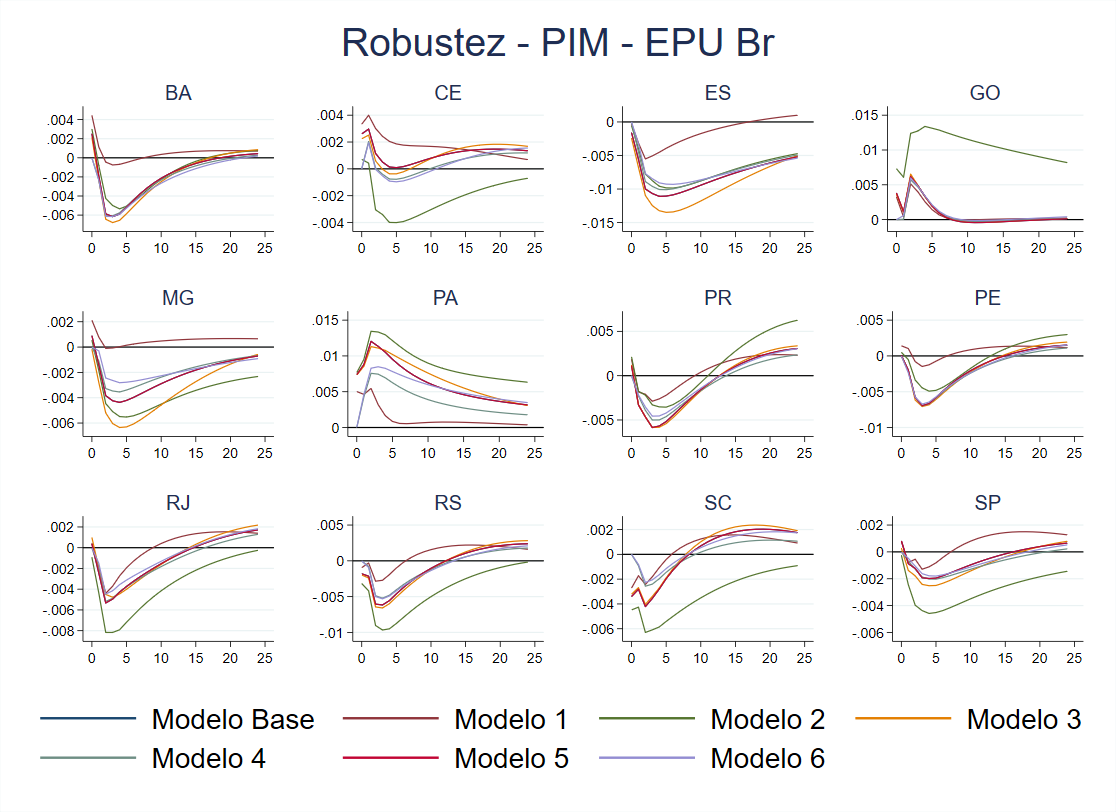
\includegraphics[height=0.65\textheight]{Figs/Robusteness/IRF_EPU_PIM_robustness.png}
    \end{center}
    \label{fig:IRF_EPU_PIM_robustness} \footnotesize
Fonte: Elaboração própria. Nota: Respostas estaduais após o choque de um desvio padrão na medida de incerteza. Os números do gráfico estão descritos em valores absolutos. 
\end{figure}
\end{frame}

\begin{frame}{Robustez - GEPU - IBCR}
\begin{figure}[htb!]
    \caption{\footnotesize Robustez - IBCR após um choque da medida de incerteza GEPU}
    \begin{center}
        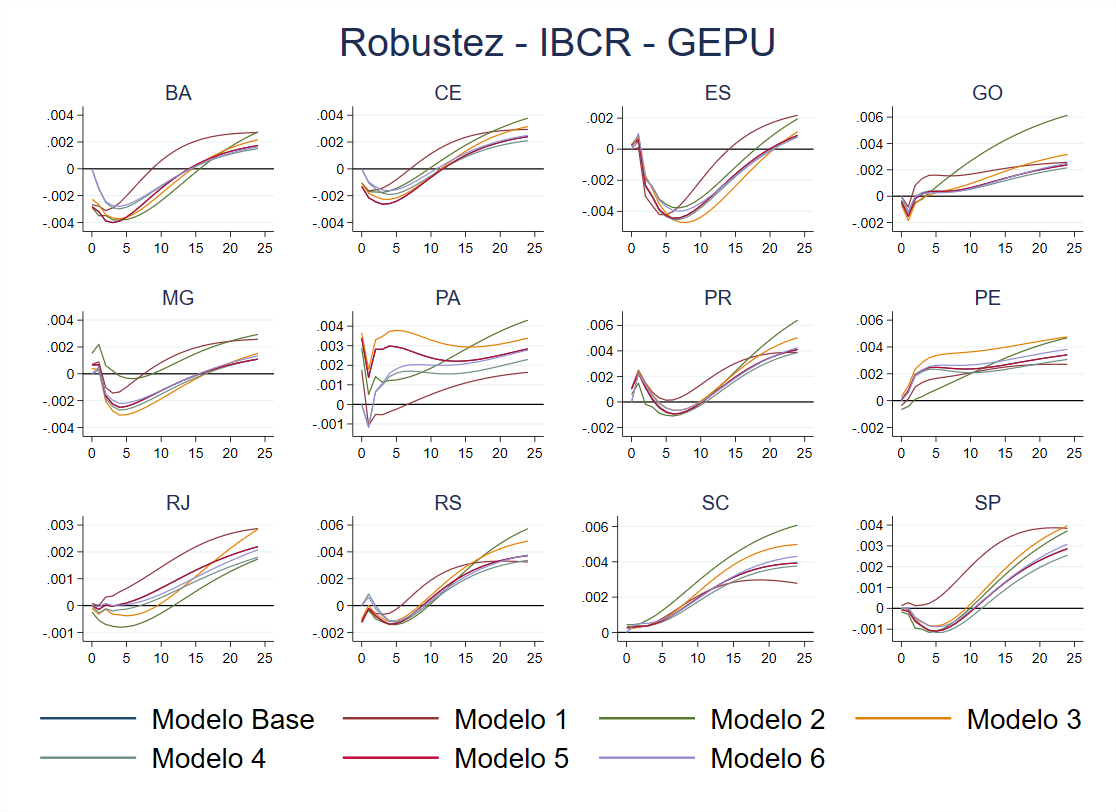
\includegraphics[height=0.65\textheight]{Figs/Robusteness/IRF_GEPU_IBCR_robustness.png}
    \end{center}
    \label{fig:IRF_GEPU_IBCR_robustness} \footnotesize
Fonte: Elaboração própria. Nota: Respostas estaduais após o choque de um desvio padrão na medida de incerteza. Os números do gráfico estão descritos em valores absolutos. 
\end{figure}
\end{frame}

\begin{frame}{Robustez - GEPU - PIM}
\begin{figure}[htb!]
    \caption{\footnotesize Robustez - PIM após um choque da medida de incerteza GEPU}
    \begin{center}
        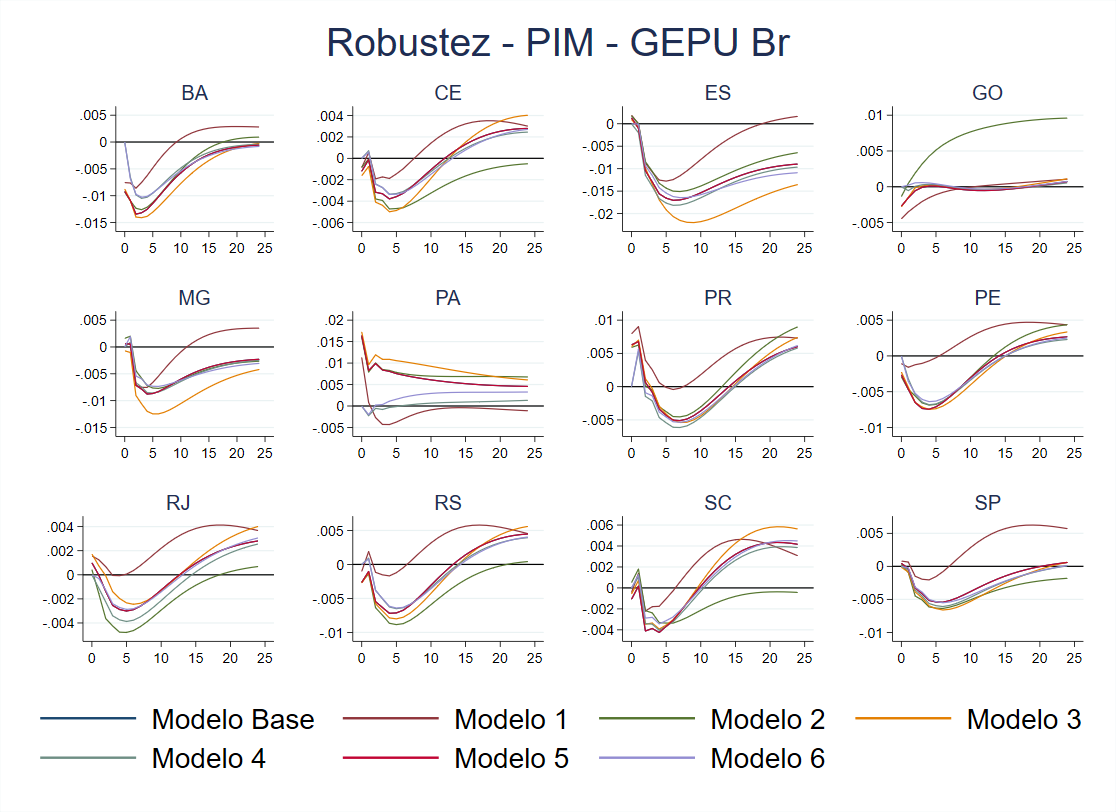
\includegraphics[height=0.65\textheight]{Figs/Robusteness/IRF_GEPU_PIM_robustness.png}
    \end{center}
    \label{fig:IRF_GEPU_PIM_robustness} \footnotesize
Fonte: Elaboração própria. Nota: Respostas estaduais após o choque de um desvio padrão na medida de incerteza. Os números do gráfico estão descritos em valores absolutos. 
\end{figure}
\end{frame}

\end{document}



